\documentclass[tikz]{standalone}
\usetikzlibrary{shapes.geometric, positioning}
\begin{document}
\tiny
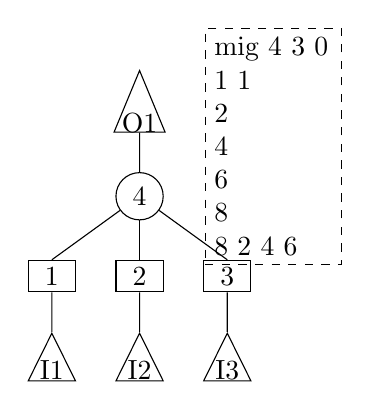
\begin{tikzpicture}[
    node distance = .5cm,
    io/.style={
        draw, isosceles triangle, isosceles triangle stretches, shape border rotate=90,
        inner sep=0pt, minimum width=.6cm, minimum height=.5cm
    },
    maj/.style={
        draw, circle, inner sep=0pt, minimum size=.6cm
    },
    pi/.style={
        draw, rectangle, inner sep=0pt, minimum width=.6cm, minimum height=.4cm,
    },
    circ/.style={
        fill, circle, inner sep=0pt, minimum size=1.8pt,
    },
]

    \node[io](o0){O1};
    \node[maj,below=of o0](m1){4};
    \node[pi,below=of m1](p2){2};
    \node[pi,left=of p2](p1){1};
    \node[pi,right=of p2](p3){3};
    \node[io,below=of p1](i1){I1};
    \node[io,below=of p2](i2){I2};
    \node[io,below=of p3](i3){I3};

    \draw (o0) to (m1);
    \draw (m1) to (p1.north);
    \draw (m1) to (p2);
    \draw (m1) to (p3.north);

    % \draw (p1) to node[circ, pos=0]{}(i1);
    \draw (p1) to (i1);
    \draw (p2) to (i2);
    \draw (p3) to (i3);

    \node[text width=1.5cm, draw, rectangle, dashed] at (1.7,-.3) {
        mig 4 3 0 1 1\\
        2\\
        4\\
        6\\
        8\\
        8 2 4 6
    };

\end{tikzpicture}
\end{document}
